\chapter{Introduzione}
\label{cha:Introduzione}

\section{Cosa determina le prestazioni di un calcolatore}
\label{sec:cosaDeterminaPrestazioni}

Un'architettura di elaborazione\footnote{Faremo costantemente riferimento al modello basato sulla macchina di Von Neumann.} è costituita da tre elementi fondamentali:
\begin{itemize}
\item l'\textbf{ISA} (\textit{Instruction Stack Architecture}), ovvero il set di istruzioni computabile dalla macchina;
\item la \textbf{struttura} (v. esempio in figura \ref{fig:strutturaSchematica}), cioè l'insieme di blocchi interconnessi fra loro che realizza il principio di funzionamento del sistema;
\begin{figure}[!h]
\centering
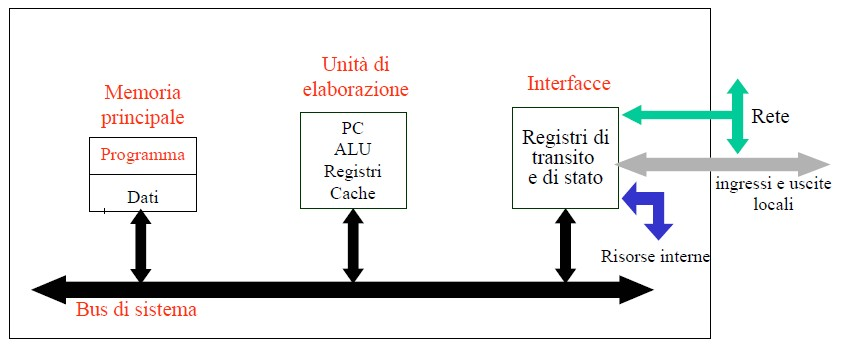
\includegraphics[width=0.8\columnwidth]{img/strutturaSchematica}
\caption{Una schematizzazione essenziale della struttura di un calcolatore}
\label{fig:strutturaSchematica}
\end{figure}
\item la \textbf{realizzazione circuitale} del sistema, cioè com'è fatto "'elettronicamente'".
\end{itemize}

Questi tre elementi impattano significativamente sulle prestazioni del nostro elaboratore, quantificabili attraverso il parametro $CPU_{time}$, cioè il tempo che impiega la macchina ad eseguire un certo \textit{task}:
\[
CPU_{time} = N_{istruzioni} \cdot CPI_{medio} \cdot T_{clock}
\]
Il numero di istruzioni ($N_{istruzioni}$) dipende dell'ISA, il $CPI_{medio}$ dalla struttura hardware del nostro sistema, il $T_{clock}$ (periodo di clock) dalla tecnologia di realizzazione (cioè dall'elettronica sottostante la fabbricazione dell'hardware).

Tecnologia e struttura interna evolvono nell'ottica di aumentare le prestazioni e ridurre il consumo/operazione
elementare. In particolare, si cerca di trovare il miglior compromesso fra potenza e consumo tramite i seguenti accorgimenti:
\begin{itemize}
\item riduzione delle tensioni di alimentazione;
\item definizione di diversi stati di funzionamento in modo da
alimentare selettivamente a divisione di tempo solo i blocchi
istante per istante necessari;
\item variazione della frequenza di funzionamento in funzione del
carico computazionale;
\item variazione della tensione di alimentazione in funzione della
frequenza istantanea di funzionamento;
\item \textit{Power management} esteso all'intero sistema, non solo alla
CPU.
\end{itemize}


\subsection{L'ISA}
\label{sec:isa}

Il linguaggio macchina (L.M.) (detto anche \textit{instruction set architecture} - ISA) è il livello dell'architettura della CPU visibile a chi sviluppa i compilatori e a chi programma in \textit{assembler}. L'ISA è costituita dall'insieme delle istruzioni eseguibili e dal loro formato binario. Con le istruzioni del linguaggio macchina si accede alle risorse interne del calcolatore (memoria, registri, tabelle e descrittori, variabili di stato, \textit{flag}, etc\ldots). Tra le risorse interne al calcolatore, solo quelle accessibili attraverso l'ISA possono essere rese visibili e controllabili dal software.

Per comodità in generale non rappresenteremo le istruzioni macchina con zeri e uni (cioè come vengono viste dal calcolatore), né con cifre esadecimali in forma simbolica; il linguaggio che useremo per rappresentare simbolicamente le istruzioni del linguaggio macchina è l'\textit{assembler}.

Le istruzioni prese in pasto da un calcolatore\footnote{In questo paragrafo faremo riferimento all'Intel 8086/8088 oppure al DLX.} hanno una struttura del tipo:
\begin{verbatim}
ADD   ALFA[DI+BX], AL
\end{verbatim}
In questo caso DI+BX è l'indice di ALFA, che è un vettore: l'operazione effettuata consiste nel sommare alla quantità presente in ALFA[DI+BX] (operando in memoria) la quantità AL. Con ALFA[DI+BX] indichiamo simbolicamente una posizione in memoria; la memoria, nell'8088, è di 1 MB ($20^{20}$ bit) ed è "'puntata'" da DS (\textit{data segment}, vedi fig. \ref{fig:DSmemoria}), vettore di 20 bit con i 4 bit meno significativi posti a 0: questo significa che è possibile indirizzare le celle di memoria, ampie $2^4 = 16$ byte ciascuna e dette \textit{paragrafi}, con soli 16 bit (4 cifre esadecimali) dei 20 totali.
\begin{figure}[!h]
\centering
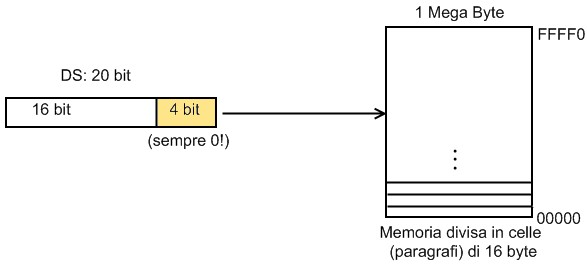
\includegraphics[width=0.7\columnwidth]{img/DSmemoria}
\caption{Struttura della memoria e suddivisione in paragrafi}
\label{fig:DSmemoria}
\end{figure}

Un'altra possibile suddivisione logica della memoria è quella in pagine, ovvero in $2^8$ blocchi di $2^{12}$ byte (vedi fig. \ref{fig:pagineParagrafi}).

\begin{figure}[!h]
\centering
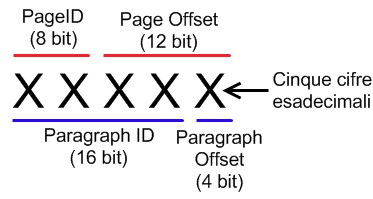
\includegraphics[width=0.4\columnwidth]{img/pagineParagrafi}
\caption{\textit{Base} e \textit{offset} per pagine e paragrafi}
\label{fig:pagineParagrafi}
\end{figure}

Si noti che la divisione in paragrafi e in pagine implica:
\begin{itemize}
\item un metodo di indirizzamento \textit{base} (indirizzo iniziale della cella di memoria) + \textit{offset} (indirizzo all'interno della cella);
\item che è possibile far sì che l'indirizzo di un blocco sia sempre un multiplo della dimensione del blocco stesso (\textit{indirizzi allineati}); questo comporta che, se prendiamo in considerazione il DLX (4 GigaByte di memoria da indirizzare, indirizzi di 32 bit), non necessiteremo di un sommatore a 32 bit per il calcolo dell'indirizzo "'effettivo'" (\textit{base} + \textit{offset}), potendo furbescamente sfruttare il concatenamento di \textit{blockID} + \textit{offset}. \\
Esempio (DLX, $n=32$, indirizzi allineati): devo accedere a una cella di memoria individuata dal \textit{blockID} che, per definizione, ha i $k$ bit meno significativi tutti a zero, e ho bisogno dell'informazione, che chiameremo PIPPO, presente ad un certo \textit{offset} lungo $k$ bit. Per trovare l'indirizzo di PIPPO basta una semplice operazione di concatenamento:
\begin{verbatim}
ind(PIPPO) [n bit] = Block_ID [n-k bit] ## Offset [k bit]
\end{verbatim}
Se invece i blocchi non sono allineati (es. 8088, dove sia la base che l'offset sono a 16 bit, con un DS di 20 bit), oppure se l'offset è maggiore della dimensione del blocco, il sommatore è imprescindibile.
\end{itemize}

Nell'8088 l'offset è calcolato dinamicamente ed è la somma di BX + DI + ALFA (vedi fig. \ref{fig:effectiveAddress}).

\begin{figure}[!h]
\centering
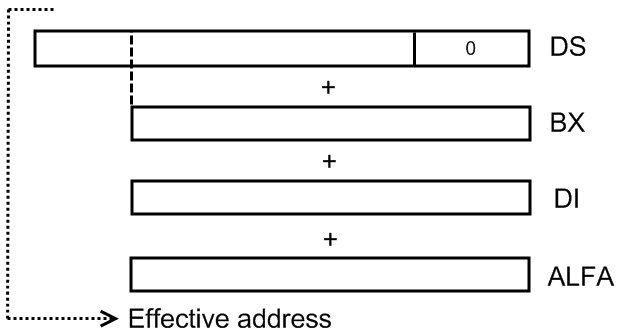
\includegraphics[width=0.5\columnwidth]{img/effectiveAddress}
\caption{Calcolo dell'\textit{effective address}}
\label{fig:effectiveAddress}
\end{figure}

\subsection{Struttura (architettura)}
\label{sec:strutturaArchitettura}

\begin{figure}[!h]
\centering
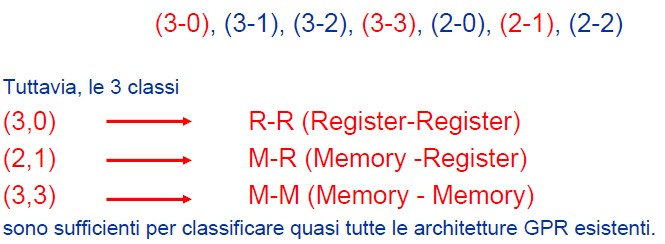
\includegraphics[width=0.7\columnwidth]{img/tipiArchitetture}
\caption{Schema riassuntivo della nomenclatura per tipologie d'architettura}
\label{fig:tipiArchitettura}
\end{figure}

Una macchina che fa uso di due operandi espliciti e di uno in memoria viene detta avente architettura 2-1. 
Esempio di istruzione di macchina 2-1 (detta anche M-R, memoria-registro): 
\begin{verbatim}
ADD   ALFA[DI+BX], AL
\end{verbatim}
Con una singola riga di codice effettuiamo una relativamente numerosa serie di operazioni elementari (memorizzazione, \textit{fetch}, somme, etc\ldots), le quali richiedono molti clock per essere eseguite; dunque:
\[
CPI_{medio}~~ \text{(clock per instruction: ALTO)} ~~~~~~~~~ N_{istruzioni}~~ \text{(numero di istruzioni: BASSO)}
\]
Si parla quindi di architettura CISC (\textit{Complex Instruction Set Computer}). \\

Il DLX ha invece un'architettura 3-0 (detta anche R-R, registro-registro), con istruzioni aventi tre operandi espliciti e nessuno in memoria:
\begin{verbatim}
ADD R5, R6, R7
\end{verbatim}
Per prelevare e depositare in memoria ci si appoggia quindi alle istruzioni di LOAD e STORE. \\

L'architettura influisce tantissimo sia sulle prestazioni che sul generale funzionamento del calcolatore: infine, con una stessa ISA possono sussistere strutture diversissime (ad esempio può essere più o meno realizzabile la \textit{pipeline} piuttosto che la struttura ad esecuzione sequenziale, etc\ldots).

\section{Tipi di istruzioni}
\label{sec:tipiIstruzioni}

In questo paragrafo considereremo l'architettura del DLX ($2^{32}$ byte di indirizzamento).

\begin{figure}[!h]
\centering
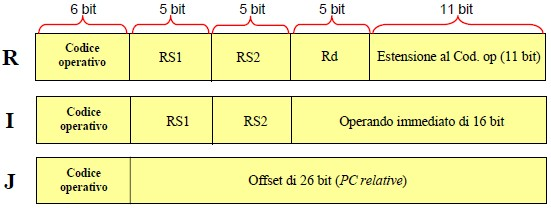
\includegraphics[width=0.65\columnwidth]{img/TipiIstruzioni}
\caption{Tipologie d'istruzione}
\label{fig:TipiIstruzioni}
\end{figure}
\begin{figure}[!h]
\centering
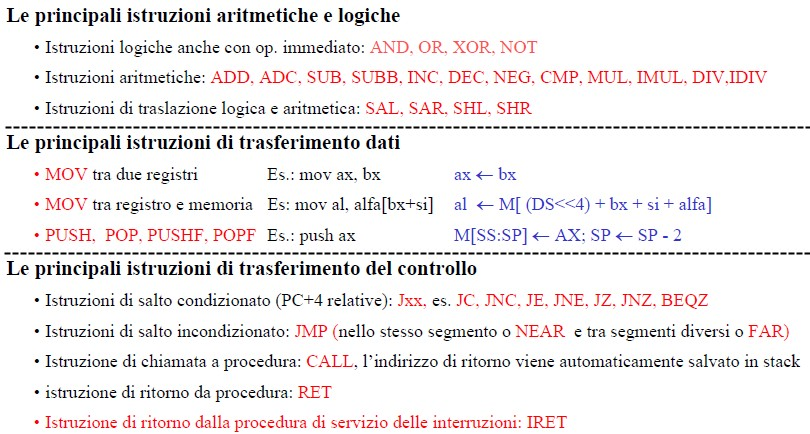
\includegraphics[width=\columnwidth]{img/listaistruzioni}
\caption{Schema di massima dei principali tipi di istruzioni}
\label{fig:listaistruzioni}
\end{figure}

\subsection{Di tipo R}
\label{sec:tipoR}

Si tratta delle tipiche istruzioni ALU, in cui sono coinvolti tre registri. Esempio:
\begin{verbatim}
ADD   R1, R2, R3
\end{verbatim}

\subsection{Di tipo I}
\label{sec:tipoI}

Sono le istruzioni con operando immediato (cui sono riservati 16 bit in complemento a 2, per un range - quindi - che va da -32K a 32K-1), come
\begin{itemize}
\item \textit{Load}/\textit{Store}. Ad esempio:
\begin{verbatim}
LB    R5, 20(R6)
\end{verbatim}
Questa istruzione\footnote{Equivalente a 
\[
R5_{[7\ldots 0]} \Leftarrow M[R6+20]
\]} mette in R5 il contenuto della cella di memoria il cui indirizzo è il contenuto del registro R6 incrementato di 20.
Oppure:
\begin{verbatim}
LDRS   ALFA(R6)
\end{verbatim}
ALFA è detta \textit{parte fissa}, mentre il contenuto di R6 è la \textit{parte variabile}: quel che si fa è accedere all'R6-simo elemento del vettore ALFA ed effettuarne il \textit{load}.
\item \textit{Branch condizionate}, ovvero salto \textbf{condizionato}. Esempio\footnote{Si tratta di una \textit{Branch Not Equal Zero}: in pratica, se in PIPPO vi è il valore 3, dobbiamo andare a PC+3 (per questo si dice che è un'istruzione \textit{PC-relative}).}
\begin{verbatim}
BNEZ   R5, PIPPO
\end{verbatim}
Altri esempi (\textit{Branch Not Equal Zero})\footnote{Se R10 è diverso da 0 saltiamo a PIPPO.}:
\begin{verbatim}
BNEQZ   R10, PIPPO
\end{verbatim}
Che è equivalente a (\textit{Jump Equal})\footnote{Se R5=R6 saltiamo a PIPPO.}
\begin{verbatim}
JEQ    R5, R6, PIPPO
\end{verbatim}
se R10 è stato ricavato con questa istruzione (\textit{Set Equal Zero})\footnote{Mettiamo in R10 il risultato del confronto fra gli operandi R5 e R6.}:
\begin{verbatim}
SEQ    R10, R5, R6
\end{verbatim}

\item \textit{Jump Register} (JR);
\item \textit{Jump and Link register} (JALR);
\item ALU con operando immediato, ad esempio:
\begin{verbatim}
ADDI   R1, R2, 3
\end{verbatim}
Per questo tipo di operazioni viene coinvolta la ALU, che prende in pasto due operandi da 32 bit: siccome l'operando immediato è una quantità a 16 bit, i rimanenti bit sono rappresentati dal bit del segno ripetuto 16 volte.
\end{itemize}

\subsection{Di tipo J}
\label{sec:tipoJ}

Si tratta di istruzioni di \textit{jump} (salto \textbf{incondizionato}), ancora una volta \textit{PC-relative} con l'operando immediato presente nella finestra\footnote{Ampia 64 MB e centrata sul PC.}:
\[
-2^{25} \Rightarrow 2^{25}-1
\]
Quando è necessario effettuare un salto (\textit{jump}) l'indirizzo di ritorno viene salvato nel registro R31 ma, se per qualche motivo nel frattempo venisse eseguita un'altra procedura, l'indirizzo di ritorno in R31 verrebbe sovrascritto e noi saremmo fregati. Quanto detto si riflette nell'assenza del cosiddetto \textit{nesting}, cosicché deve curarsene il programmatore (facendo uso, ad esempio, di altri registri come R30). Se teniamo conto di questo aspetto, come ci regoliamo con gli \textit{interrupt}? Gli \textit{interrupt} sono chiamate a procedure "'implicite'", scatenate da un evento o un dispositivo esterno (come ad esempio una periferica): l'indirizzo di ritorno, in questo caso, non viene salvato in R31 bensì in IAR(\textit{Interrupt Address Register}). 
IAR e R31 sono quindi i due registri deputati al salvataggio degli indirizzi di ritorno.

Come facciamo per regolare il ritorno dalle eccezioni (ad es. divisione per zero, al sopraggiungere della quale la CPU si arrabbia e si sfoga sull'utente generando - appunto - un'eccezione)? Esiste un'istruzione ad-hoc
\begin{verbatim}
RFE   (Return From Exception)
\end{verbatim}
all'esecuzione della quale si salva l'indirizzo corrente in IAR. 
